% Options for packages loaded elsewhere
\PassOptionsToPackage{unicode}{hyperref}
\PassOptionsToPackage{hyphens}{url}
\PassOptionsToPackage{dvipsnames,svgnames*,x11names*}{xcolor}
%
\documentclass[
  11pt,
]{article}
\usepackage[]{mathpazo}
\usepackage{amsmath}
\usepackage{ifxetex,ifluatex}
\ifnum 0\ifxetex 1\fi\ifluatex 1\fi=0 % if pdftex
  \usepackage[T1]{fontenc}
  \usepackage[utf8]{inputenc}
  \usepackage{textcomp} % provide euro and other symbols
  \usepackage{amssymb}
\else % if luatex or xetex
  \usepackage{unicode-math}
  \defaultfontfeatures{Scale=MatchLowercase}
  \defaultfontfeatures[\rmfamily]{Ligatures=TeX,Scale=1}
\fi
% Use upquote if available, for straight quotes in verbatim environments
\IfFileExists{upquote.sty}{\usepackage{upquote}}{}
\IfFileExists{microtype.sty}{% use microtype if available
  \usepackage[]{microtype}
  \UseMicrotypeSet[protrusion]{basicmath} % disable protrusion for tt fonts
}{}
\usepackage{xcolor}
\IfFileExists{xurl.sty}{\usepackage{xurl}}{} % add URL line breaks if available
\IfFileExists{bookmark.sty}{\usepackage{bookmark}}{\usepackage{hyperref}}
\hypersetup{
  pdftitle={Supplementary Material},
  pdfauthor={Nathan I. Hoffmann, Department of Sociology, University of California, Los Angeles; Kristopher Velasco, Department of Sociology, University of Texas at Austin},
  colorlinks=true,
  linkcolor=blue,
  filecolor=Maroon,
  citecolor=Blue,
  urlcolor=Blue,
  pdfcreator={LaTeX via pandoc}}
\urlstyle{same} % disable monospaced font for URLs
\usepackage[margin=1in]{geometry}
\usepackage{longtable,booktabs}
\usepackage{calc} % for calculating minipage widths
% Correct order of tables after \paragraph or \subparagraph
\usepackage{etoolbox}
\makeatletter
\patchcmd\longtable{\par}{\if@noskipsec\mbox{}\fi\par}{}{}
\makeatother
% Allow footnotes in longtable head/foot
\IfFileExists{footnotehyper.sty}{\usepackage{footnotehyper}}{\usepackage{footnote}}
\makesavenoteenv{longtable}
\usepackage{graphicx}
\makeatletter
\def\maxwidth{\ifdim\Gin@nat@width>\linewidth\linewidth\else\Gin@nat@width\fi}
\def\maxheight{\ifdim\Gin@nat@height>\textheight\textheight\else\Gin@nat@height\fi}
\makeatother
% Scale images if necessary, so that they will not overflow the page
% margins by default, and it is still possible to overwrite the defaults
% using explicit options in \includegraphics[width, height, ...]{}
\setkeys{Gin}{width=\maxwidth,height=\maxheight,keepaspectratio}
% Set default figure placement to htbp
\makeatletter
\def\fps@figure{htbp}
\makeatother
\setlength{\emergencystretch}{3em} % prevent overfull lines
\providecommand{\tightlist}{%
  \setlength{\itemsep}{0pt}\setlength{\parskip}{0pt}}
\setcounter{secnumdepth}{5}
\usepackage{fancyhdr}
\pagestyle{fancy}
\setlength{\headheight}{13.6pt}
\rhead{\textit{Hoffmann and Velasco}}
\usepackage{booktabs}
\usepackage{longtable}
\usepackage{array}
\usepackage{multirow}
\usepackage{wrapfig}
\usepackage{float}
\usepackage{colortbl}
\usepackage{pdflscape}
\usepackage{tabu}
\usepackage{threeparttable}
\usepackage{threeparttablex}
\usepackage[normalem]{ulem}
\usepackage{makecell}
\usepackage{xcolor}
\ifluatex
  \usepackage{selnolig}  % disable illegal ligatures
\fi
\newlength{\cslhangindent}
\setlength{\cslhangindent}{1.5em}
\newlength{\csllabelwidth}
\setlength{\csllabelwidth}{3em}
\newenvironment{CSLReferences}[2] % #1 hanging-ident, #2 entry spacing
 {% don't indent paragraphs
  \setlength{\parindent}{0pt}
  % turn on hanging indent if param 1 is 1
  \ifodd #1 \everypar{\setlength{\hangindent}{\cslhangindent}}\ignorespaces\fi
  % set entry spacing
  \ifnum #2 > 0
  \setlength{\parskip}{#2\baselineskip}
  \fi
 }%
 {}
\usepackage{calc}
\newcommand{\CSLBlock}[1]{#1\hfill\break}
\newcommand{\CSLLeftMargin}[1]{\parbox[t]{\csllabelwidth}{#1}}
\newcommand{\CSLRightInline}[1]{\parbox[t]{\linewidth - \csllabelwidth}{#1}\break}
\newcommand{\CSLIndent}[1]{\hspace{\cslhangindent}#1}

\title{Supplementary Material}
\usepackage{etoolbox}
\makeatletter
\providecommand{\subtitle}[1]{% add subtitle to \maketitle
  \apptocmd{\@title}{\par {\large #1 \par}}{}{}
}
\makeatother
\subtitle{Making Migration Sexy}
\author{Nathan I. Hoffmann, Department of Sociology, University of California, Los Angeles \and Kristopher Velasco, Department of Sociology, University of Texas at Austin}
\date{May 31, 2021}

\begin{document}
\maketitle

{
\hypersetup{linkcolor=}
\setcounter{tocdepth}{2}
\tableofcontents
}
\hypertarget{additional-descriptive-analyses}{%
\section{Additional descriptive analyses}\label{additional-descriptive-analyses}}

\begin{table}

\caption{\label{tab:desc-top1}Top 10 sending countries of immigrants in same-sex couples in the American Community Survey 2008-2019}
\centering
\begin{tabular}[t]{lr}
\toprule
Birth country & n\\
\midrule
Mexico & 1170\\
Philippines & 525\\
Canada & 419\\
Brazil & 321\\
China & 311\\
\addlinespace
Cuba & 288\\
India & 264\\
Colombia & 249\\
United Kingdom, ns & 248\\
Germany & 176\\
\bottomrule
\end{tabular}
\end{table}

\begin{table}

\caption{\label{tab:desc-top2}Top 10 sending countries of immigrants in different-sex couples in the American Community Survey 2008-2019}
\centering
\begin{tabular}[t]{lr}
\toprule
Birth country & n\\
\midrule
Mexico & 201087\\
India & 100008\\
China & 63686\\
Philippines & 50108\\
Vietnam & 28318\\
\addlinespace
Canada & 27776\\
Korea & 24076\\
Cuba & 23933\\
El Salvador & 18777\\
Colombia & 17341\\
\bottomrule
\end{tabular}
\end{table}

\begin{figure}
\centering
\includegraphics{ssimm_supp_small_files/figure-latex/desc-fig-1.pdf}
\caption{\label{fig:desc-fig}Additional descriptive statistics for immigrants in couples 2008-2019, with survey weights and 95\% confidence intervals. All currency in 1000s of 1999 dollars.}
\end{figure}

\newpage

\hypertarget{alternate-specifications-of-country-proportion-models}{%
\section{Alternate specifications of country proportion models}\label{alternate-specifications-of-country-proportion-models}}

\begin{table}[!htbp] \centering 
  \caption{Alternate Specifications of OLS regressions of percent of immigrants in same-sex couples by year of immigration and country of origin, using only proportions of married couples or couples with one immigrant and one U.S.-born citizen. Country-clustered standard errors shown in parentheses. Country controls include population-weighted distance, contiguous border, common official language, common ethnic language, colonial relationship, wage differential, unemployment differential, proportion same-country stock, and Polity 5 measure of democracy.} 
  \label{tab:country-props-alt} 
\begin{tabular}{@{\extracolsep{5pt}}lcccccc} 
\\[-1.8ex]\hline 
\hline \\[-1.8ex] 
 & \multicolumn{6}{c}{\textit{Dependent variable:}} \\ 
\cline{2-7} 
\\[-1.8ex] & \multicolumn{3}{c}{Married} & \multicolumn{3}{c}{One Immigrant} \\ 
\\[-1.8ex] & (1) & (2) & (3) & (4) & (5) & (6)\\ 
\hline \\[-1.8ex] 
 Country LGBT policy score & 0.076$^{***}$ & 0.041$^{†}$ & 0.001 & 0.009 & 0.003 & $-$0.010 \\ 
  & (0.022) & (0.024) & (0.028) & (0.008) & (0.009) & (0.010) \\ 
  & & & & & & \\ 
 Post-2013 &  & 0.350$^{***}$ & 0.200$^{*}$ &  & 0.057$^{†}$ & 0.009 \\ 
  &  & (0.085) & (0.100) &  & (0.030) & (0.035) \\ 
  & & & & & & \\ 
 Country score × Post-2013 &  &  & 0.070$^{**}$ &  &  & 0.023$^{**}$ \\ 
  &  &  & (0.025) &  &  & (0.009) \\ 
  & & & & & & \\ 
\hline \\[-1.8ex] 
Country controls? & yes & yes & yes & yes & yes & yes \\ 
Country FEs? & yes & yes & yes & yes & yes & yes \\ 
Observations & 3,281 & 3,281 & 3,281 & 3,281 & 3,281 & 3,281 \\ 
\hline 
\hline \\[-1.8ex] 
\multicolumn{7}{l}{Note: †p<0.1; *p<0.05; **p<0.01; ***p<0.001} \\ 
\multicolumn{7}{l}{Source: American Community Survey 2008-2019} \\ 
\end{tabular} 
\end{table}

\newpage

\hypertarget{relative-immmigrant-population-weighted-regressions}{%
\section{Relative immmigrant population-weighted regressions}\label{relative-immmigrant-population-weighted-regressions}}

We perform the same regressions with proportion in same-sex couples by country or state, but weighted by the relative size of the immigrant stock.

\begin{table}[!htbp] \centering 
  \caption{Weighted OLS regressions of percent of immigrants in same-sex couples by year of immigration and country of origin. Country-clustered standard errors shown in parentheses.} 
  \label{tab:country-props} 
\begin{tabular}{@{\extracolsep{5pt}}lccccc} 
\\[-1.8ex]\hline 
\hline \\[-1.8ex] 
 & \multicolumn{5}{c}{\textit{Dependent variable:}} \\ 
\cline{2-6} 
\\[-1.8ex] & \multicolumn{5}{c}{Percent in same-sex couples by country-year} \\ 
\\[-1.8ex] & (1) & (2) & (3) & (4) & (5)\\ 
\hline \\[-1.8ex] 
 Country LGB policy score & 0.057$^{***}$ & 0.051$^{***}$ & 0.038$^{***}$ & 0.020$^{*}$ & 0.001 \\ 
  & (0.005) & (0.006) & (0.007) & (0.008) & (0.009) \\ 
  & & & & & \\ 
 Post-2013 &  &  &  & 0.180$^{***}$ & 0.062 \\ 
  &  &  &  & (0.032) & (0.044) \\ 
  & & & & & \\ 
 Country score × Post-2013 &  &  &  &  & 0.038$^{***}$ \\ 
  &  &  &  &  & (0.010) \\ 
  & & & & & \\ 
\hline \\[-1.8ex] 
Country controls? & no & yes & yes & yes & yes \\ 
Country FEs? & no & no & yes & yes & yes \\ 
Observations & 3,281 & 3,281 & 3,281 & 3,281 & 3,281 \\ 
\hline 
\hline \\[-1.8ex] 
\multicolumn{6}{l}{Note: †p<0.1; *p<0.05; **p<0.01; ***p<0.001} \\ 
\multicolumn{6}{l}{Source: American Community Survey 2008-2019} \\ 
\end{tabular} 
\end{table}

\begin{table}[!htbp] \centering 
  \caption{Weighted regression of percent same-sex in by country of origin, U.S. state, and survey year. Country-clustered standard errors are shown in parentheses.} 
  \label{tab:state-props} 
\begin{tabular}{@{\extracolsep{5pt}}lcccccc} 
\\[-1.8ex]\hline 
\hline \\[-1.8ex] 
 & \multicolumn{6}{c}{\textit{Dependent variable:}} \\ 
\cline{2-7} 
\\[-1.8ex] & \multicolumn{6}{c}{Percent in same-sex couples by state-country-year} \\ 
\\[-1.8ex] & (1) & (2) & (3) & (4) & (5) & (6)\\ 
\hline \\[-1.8ex] 
 State LGB policy score & 0.050$^{***}$ & 0.048$^{***}$ & 0.027 & 0.018 & 0.005 & 0.006 \\ 
  & (0.006) & (0.006) & (0.020) & (0.021) & (0.023) & (0.024) \\ 
  & & & & & & \\ 
 Country LGB policy score &  & 0.082$^{***}$ & 0.078$^{***}$ & 0.078$^{*}$ & 0.073$^{*}$ & 0.023 \\ 
  &  & (0.009) & (0.009) & (0.031) & (0.032) & (0.043) \\ 
  & & & & & & \\ 
 Post-2013 &  &  &  &  & 0.079 & 0.007 \\ 
  &  &  &  &  & (0.060) & (0.073) \\ 
  & & & & & & \\ 
 Country score × Post-2013 &  &  &  &  &  & 0.040$^{†}$ \\ 
  &  &  &  &  &  & (0.023) \\ 
  & & & & & & \\ 
\hline \\[-1.8ex] 
State controls and FEs? & no & no & yes & yes & yes & yes \\ 
Country controls and FEs? & no & no & no & yes & yes & yes \\ 
Observations & 35,868 & 35,868 & 35,868 & 35,868 & 35,868 & 35,868 \\ 
\hline 
\hline \\[-1.8ex] 
\multicolumn{7}{l}{Note: †p<0.1; *p<0.05; **p<0.01; ***p<0.001} \\ 
\multicolumn{7}{l}{Source: American Community Survey 2008-2019} \\ 
\end{tabular} 
\end{table}

\newpage

\hypertarget{ols-models-of-individual-state-of-residence}{%
\section{OLS models of individual state of residence}\label{ols-models-of-individual-state-of-residence}}

\begin{table}[!htbp] \centering 
  \caption{Individual OLS analysis of state policy score. Country-clustered standard errors are shown in parentheses. Individual controls include sex, age, education, number of children, log(income), indicator for no income, and year of immigration, which are all interacted with the indicator for same-sex couple.} 
  \label{tab:ols} 
\begin{tabular}{@{\extracolsep{5pt}}lcccc} 
\\[-1.8ex]\hline 
\hline \\[-1.8ex] 
 & \multicolumn{4}{c}{\textit{Dependent variable:}} \\ 
\cline{2-5} 
\\[-1.8ex] & \multicolumn{4}{c}{Binned state LGB policy score} \\ 
\\[-1.8ex] & (1) & (2) & (3) & (4)\\ 
\hline \\[-1.8ex] 
 Same-sex & 0.530$^{***}$ & 0.380$^{***}$ & 25.000$^{**}$ & 22.000$^{***}$ \\ 
  & (0.029) & (0.041) & (9.600) & (6.400) \\ 
  & & & & \\ 
 Country LGB policy score &  & $-$0.036$^{***}$ & $-$0.058$^{***}$ & 0.020$^{***}$ \\ 
  &  & (0.004) & (0.004) & (0.003) \\ 
  & & & & \\ 
 Same-sex × country score &  & 0.070$^{***}$ & 0.056$^{***}$ & $-$0.010 \\ 
  &  & (0.012) & (0.013) & (0.009) \\ 
  & & & & \\ 
\hline \\[-1.8ex] 
Individual controls? & no & no & yes & yes \\ 
State controls and FEs? & no & no & no & yes \\ 
Country controls and FEs? & no & no & no & yes \\ 
Observations & 107,500 & 107,500 & 107,500 & 101,849 \\ 
\hline 
\hline \\[-1.8ex] 
\multicolumn{5}{l}{Note: †p<0.1; *p<0.05; **p<0.01; ***p<0.001} \\ 
\multicolumn{5}{l}{Source: American Community Survey 2008-2019} \\ 
\end{tabular} 
\end{table}

\includegraphics{ssimm_supp_small_files/figure-latex/ols-ind-sim2-1.pdf}

\newpage

\hypertarget{adjusting-proportions-based-on-empirical-mismatch-rates}{%
\section{Adjusting proportions based on empirical mismatch rates}\label{adjusting-proportions-based-on-empirical-mismatch-rates}}

\begin{table}

\caption{\label{tab:respmode}Response mode proportions for different- and same-sex couples, by year. Proportions are within couple type and year.}
\centering
\fontsize{9}{11}\selectfont
\begin{tabular}[t]{llrrrrrrrrrrrr}
\toprule
respmode & same\_sex & 2008 & 2009 & 2010 & 2011 & 2012 & 2013 & 2014 & 2015 & 2016 & 2017 & 2018 & 2019\\
\midrule
CATI/CAPI & FALSE & 0.45 & 0.44 & 0.41 & 0.42 & 0.40 & 0.36 & 0.35 & 0.34 & 0.32 & 0.29 & 0.27 & 0.24\\
Internet & FALSE & 0.00 & 0.00 & 0.00 & 0.00 & 0.00 & 0.44 & 0.46 & 0.50 & 0.53 & 0.56 & 0.59 & 0.62\\
Mail & FALSE & 0.55 & 0.56 & 0.59 & 0.58 & 0.60 & 0.20 & 0.18 & 0.17 & 0.15 & 0.15 & 0.14 & 0.14\\
CATI/CAPI & TRUE & 0.28 & 0.26 & 0.23 & 0.28 & 0.23 & 0.14 & 0.19 & 0.14 & 0.19 & 0.16 & 0.14 & 0.11\\
Internet & TRUE & 0.00 & 0.00 & 0.00 & 0.00 & 0.00 & 0.58 & 0.58 & 0.67 & 0.63 & 0.68 & 0.69 & 0.69\\
\addlinespace
Mail & TRUE & 0.72 & 0.74 & 0.77 & 0.72 & 0.77 & 0.28 & 0.22 & 0.19 & 0.19 & 0.17 & 0.17 & 0.19\\
\bottomrule
\end{tabular}
\end{table}

\begin{table}

\caption{\label{tab:mismatch}Mismatch rates from Kreider \& Lofquist (2015) and Kreider et al. (2017)}
\centering
\begin{tabular}[t]{rlllll}
\toprule
Study Year & Relationship & Mail & Internet & CAPI/CATI & Overall\\
\midrule
2010 & Married & 59\% & NA & 46\% & 57.3\%\\
2010 & Unmarried Partner & 7\% & NA & 13\% & 7\%\\
2016 & Married & 47.4\% & 22.5\% & Unknown & 35\%\\
2016 & Unmarried Partner & 5.6\% & 2.4\% & Unknown & 3.4\%\\
\bottomrule
\multicolumn{6}{l}{\rule{0pt}{1em}\textit{Source:} American Community Survey 2008-2019. Authors' calculations.}\\
\end{tabular}
\end{table}

Published papers using the ACS to study same-sex couples overwhelmingly use the method by \protect\hyperlink{ref-gates_2009}{Gates \& Steinberger} (\protect\hyperlink{ref-gates_2009}{2009}) employed our main paper to adjust for misreporting. However here we implement a novel method to adjust proportions of estimated immigrants in same-sex couples, based on the estimated mismatch rates from two U.S. Census Bureau studies. Beginning in 2019, the ACS provides explicit categories for ``Opposite-sex husband/wife/spouse,'' ``Opposite-sex unmarried partner,'' ``Same-sex husband/wife/spouse,'' and ``Same-sex unmarried partner'' (\protect\hyperlink{ref-walker_2021}{Walker \& Taylor, 2021}), so sex misreporting in the 2019 data is unlikely. Hence in most sensitivity analyses below, 2019 estimates are not adjusted for misreporting.

In a Census Bureau working paper, \protect\hyperlink{ref-kreider_2015}{Kreider \& Lofquist} (\protect\hyperlink{ref-kreider_2015}{2015}) use personal information such as names and addresses match same-sex couples from the 2010 ACS to Social Security administrative data. They find that 57 percent of married couples coded as same-sex in the ACS are coded as different-sex in the administrative data. The corresponding sex mismatch rate for unmarried same-sex couples is 7 percent. (Our data include 4,632 married and 4,428 unmarried same-sex immigrant couples.) A follow-up study (\protect\hyperlink{ref-kreider_2017}{Kreider et al., 2017}) shows that these mismatch rates appear to have fallen: In a 2016 ACS test module that included explicit categories for different- and same-sex spouses and partners, 31 percent of married and 3 percent of unmarried same-sex couples had inconsistent sex responses. This decreasing mismatch rate may be due to the greater numbers of same-sex couples openly identifying themselves as well as the growing popularity of responding to the ACS via Internet (see Supplementary Material), a response mode introduced in 2013 which is now the default (\protect\hyperlink{ref-u.s.censusbureau_2017}{U.S. Census Bureau, 2017}). In the 2016 test of the ACS, the mismatch rate for mail-in responses was 47 and 6 percent for married and unmarried same-sex couples, respectively, whereas for Internet responses they were only 22 and 2.4 percent (\protect\hyperlink{ref-kreider_2017}{Kreider et al., 2017}). A computer-assisted telephone interviewing (CATI) or computer-assisted personal interviewing (CAPI) response mode is sometimes administered as well, but the 2016 study did not assess its error rate. In the 2010 ACS, \protect\hyperlink{ref-kreider_2015}{Kreider \& Lofquist} (\protect\hyperlink{ref-kreider_2015}{2015}) find CATI/CAPI sex reporting mismatch for 46 and 13 percent for married and unmarried same-sex couples, respectively. In our sample of immigrants in same-sex couples, 2,386 responded by mail, 1,299 responded by CAPI/CATI, and 3,815 responded by Internet survey. Response mode proportions by couple type are shown in Table \ref{tab:respmode}.

Table \ref{tab:mismatch} shows the mismatch rates estimated by \protect\hyperlink{ref-kreider_2015}{Kreider \& Lofquist} (\protect\hyperlink{ref-kreider_2015}{2015}) and \protect\hyperlink{ref-kreider_2015}{Kreider \& Lofquist} (\protect\hyperlink{ref-kreider_2015}{2015}). In the supplemental analysis below (Table \ref{tab:country-props-adj}), we use these apparent mismatch rates to adjust proportions used in models in Table 3 of the main paper. Each proportion is adjusted separately by marital status and response mode. For example, all internet respondents coded as being in married same-sex couples have their final proportion reduced by 22.5\%. For mail-in responses, the proportions are reduced by the average between the two studies (53 percent for married and 6.3 percent for unmarried couples).

\begin{table}[!htbp] \centering 
  \caption{Adjusted by rates of empirical sex mismatch by married, unmarried, and response mode. OLS regressions of percent of immigrants in same-sex couples by year of immigration and country of origin, adjusted. Country-clustered standard errors shown in parentheses. Country controls include population-weighted distance, contiguous border, common official language, common ethnic language, colonial relationship, wage differential, unemployment differential, proportion same-country stock, and democracy.} 
  \label{tab:country-props-adj} 
\begin{tabular}{@{\extracolsep{5pt}}lccccc} 
\\[-1.8ex]\hline 
\hline \\[-1.8ex] 
 & \multicolumn{5}{c}{\textit{Dependent variable:}} \\ 
\cline{2-6} 
\\[-1.8ex] & \multicolumn{5}{c}{Percent in same-sex couples by country-year} \\ 
\\[-1.8ex] & (1) & (2) & (3) & (4) & (5)\\ 
\hline \\[-1.8ex] 
 Country LGBT policy score & 0.075$^{***}$ & 0.043$^{***}$ & 0.046$^{*}$ & 0.022 & $-$0.015 \\ 
  & (0.009) & (0.012) & (0.018) & (0.020) & (0.023) \\ 
  & & & & & \\ 
 Post-2013 &  &  &  & 0.240$^{***}$ & 0.110 \\ 
  &  &  &  & (0.070) & (0.082) \\ 
  & & & & & \\ 
 Country score × Post-2013 &  &  &  &  & 0.065$^{**}$ \\ 
  &  &  &  &  & (0.021) \\ 
  & & & & & \\ 
\hline \\[-1.8ex] 
Country controls? & no & yes & yes & yes & yes \\ 
Country FEs? & no & no & yes & yes & yes \\ 
Observations & 3,281 & 3,281 & 3,281 & 3,281 & 3,281 \\ 
\hline 
\hline \\[-1.8ex] 
\multicolumn{6}{l}{Note: †p<0.1; *p<0.05; **p<0.01; ***p<0.001} \\ 
\multicolumn{6}{l}{Source: American Community Survey 2008-2019} \\ 
\end{tabular} 
\end{table}

\begin{table}[!htbp] \centering 
  \caption{Adjusted by rates of empirical sex mismatch by married, unmarried, and response mode. Percent same-sex in by country of origin, U.S. state, and survey year. Country and state two-way clustered standard errors are shown in parentheses. State controls include unemployment rate and per-capita income. Country controls include population-weighted distance, contiguous border, common official language, common ethnic language, colonial relationship, wage differential, unemployment differential, proportion same-country stock, and democracy.} 
  \label{tab:state-props} 
\begin{tabular}{@{\extracolsep{5pt}}lcccccc} 
\\[-1.8ex]\hline 
\hline \\[-1.8ex] 
 & \multicolumn{6}{c}{\textit{Dependent variable:}} \\ 
\cline{2-7} 
\\[-1.8ex] & \multicolumn{6}{c}{Percent in same-sex couples by state-country-year} \\ 
\\[-1.8ex] & (1) & (2) & (3) & (4) & (5) & (6)\\ 
\hline \\[-1.8ex] 
 State LGB policy score & 0.046$^{***}$ & 0.043$^{***}$ & 0.089$^{**}$ & 0.082$^{**}$ & 0.066$^{*}$ & 0.067$^{*}$ \\ 
  & (0.008) & (0.008) & (0.028) & (0.029) & (0.032) & (0.032) \\ 
  & & & & & & \\ 
 Country LGB policy score &  & 0.072$^{***}$ & 0.067$^{***}$ & 0.120$^{**}$ & 0.110$^{**}$ & 0.034 \\ 
  &  & (0.009) & (0.009) & (0.037) & (0.038) & (0.046) \\ 
  & & & & & & \\ 
 Post-2013 &  &  &  &  & 0.099 & 0.016 \\ 
  &  &  &  &  & (0.081) & (0.085) \\ 
  & & & & & & \\ 
 Country score × Post-2013 &  &  &  &  &  & 0.060$^{**}$ \\ 
  &  &  &  &  &  & (0.020) \\ 
  & & & & & & \\ 
\hline \\[-1.8ex] 
State controls and FEs? & no & no & yes & yes & yes & yes \\ 
Country controls and FEs? & no & no & no & yes & yes & yes \\ 
Observations & 35,868 & 35,868 & 35,868 & 35,868 & 35,868 & 35,868 \\ 
\hline 
\hline \\[-1.8ex] 
\multicolumn{7}{l}{Note: †p<0.1; *p<0.05; **p<0.01; ***p<0.001} \\ 
\multicolumn{7}{l}{Source: American Community Survey 2008-2019} \\ 
\end{tabular} 
\end{table}

Figure \ref{fig:sens} takes Model 3 from the country proportions models (Table 3) and Model 4 from the state proportions models (Table 4) and reduces the proportions of same-sex couples in the data for pre-2019 data. It varies the percentage of misreported same-sex married couples from 0 to 90 percent and of unmarried couples from 0 to 14 percent. Highlighted in blue bars are the empirical mismatch rates found in the two studies by \protect\hyperlink{ref-kreider_2015}{Kreider \& Lofquist} (\protect\hyperlink{ref-kreider_2015}{2015}) and \protect\hyperlink{ref-kreider_2017}{Kreider et al.} (\protect\hyperlink{ref-kreider_2017}{2017}). We see that even extremely high misreporting rates in the pre-2019 ACS do not reduce our results to 0.

\begin{figure}
\centering
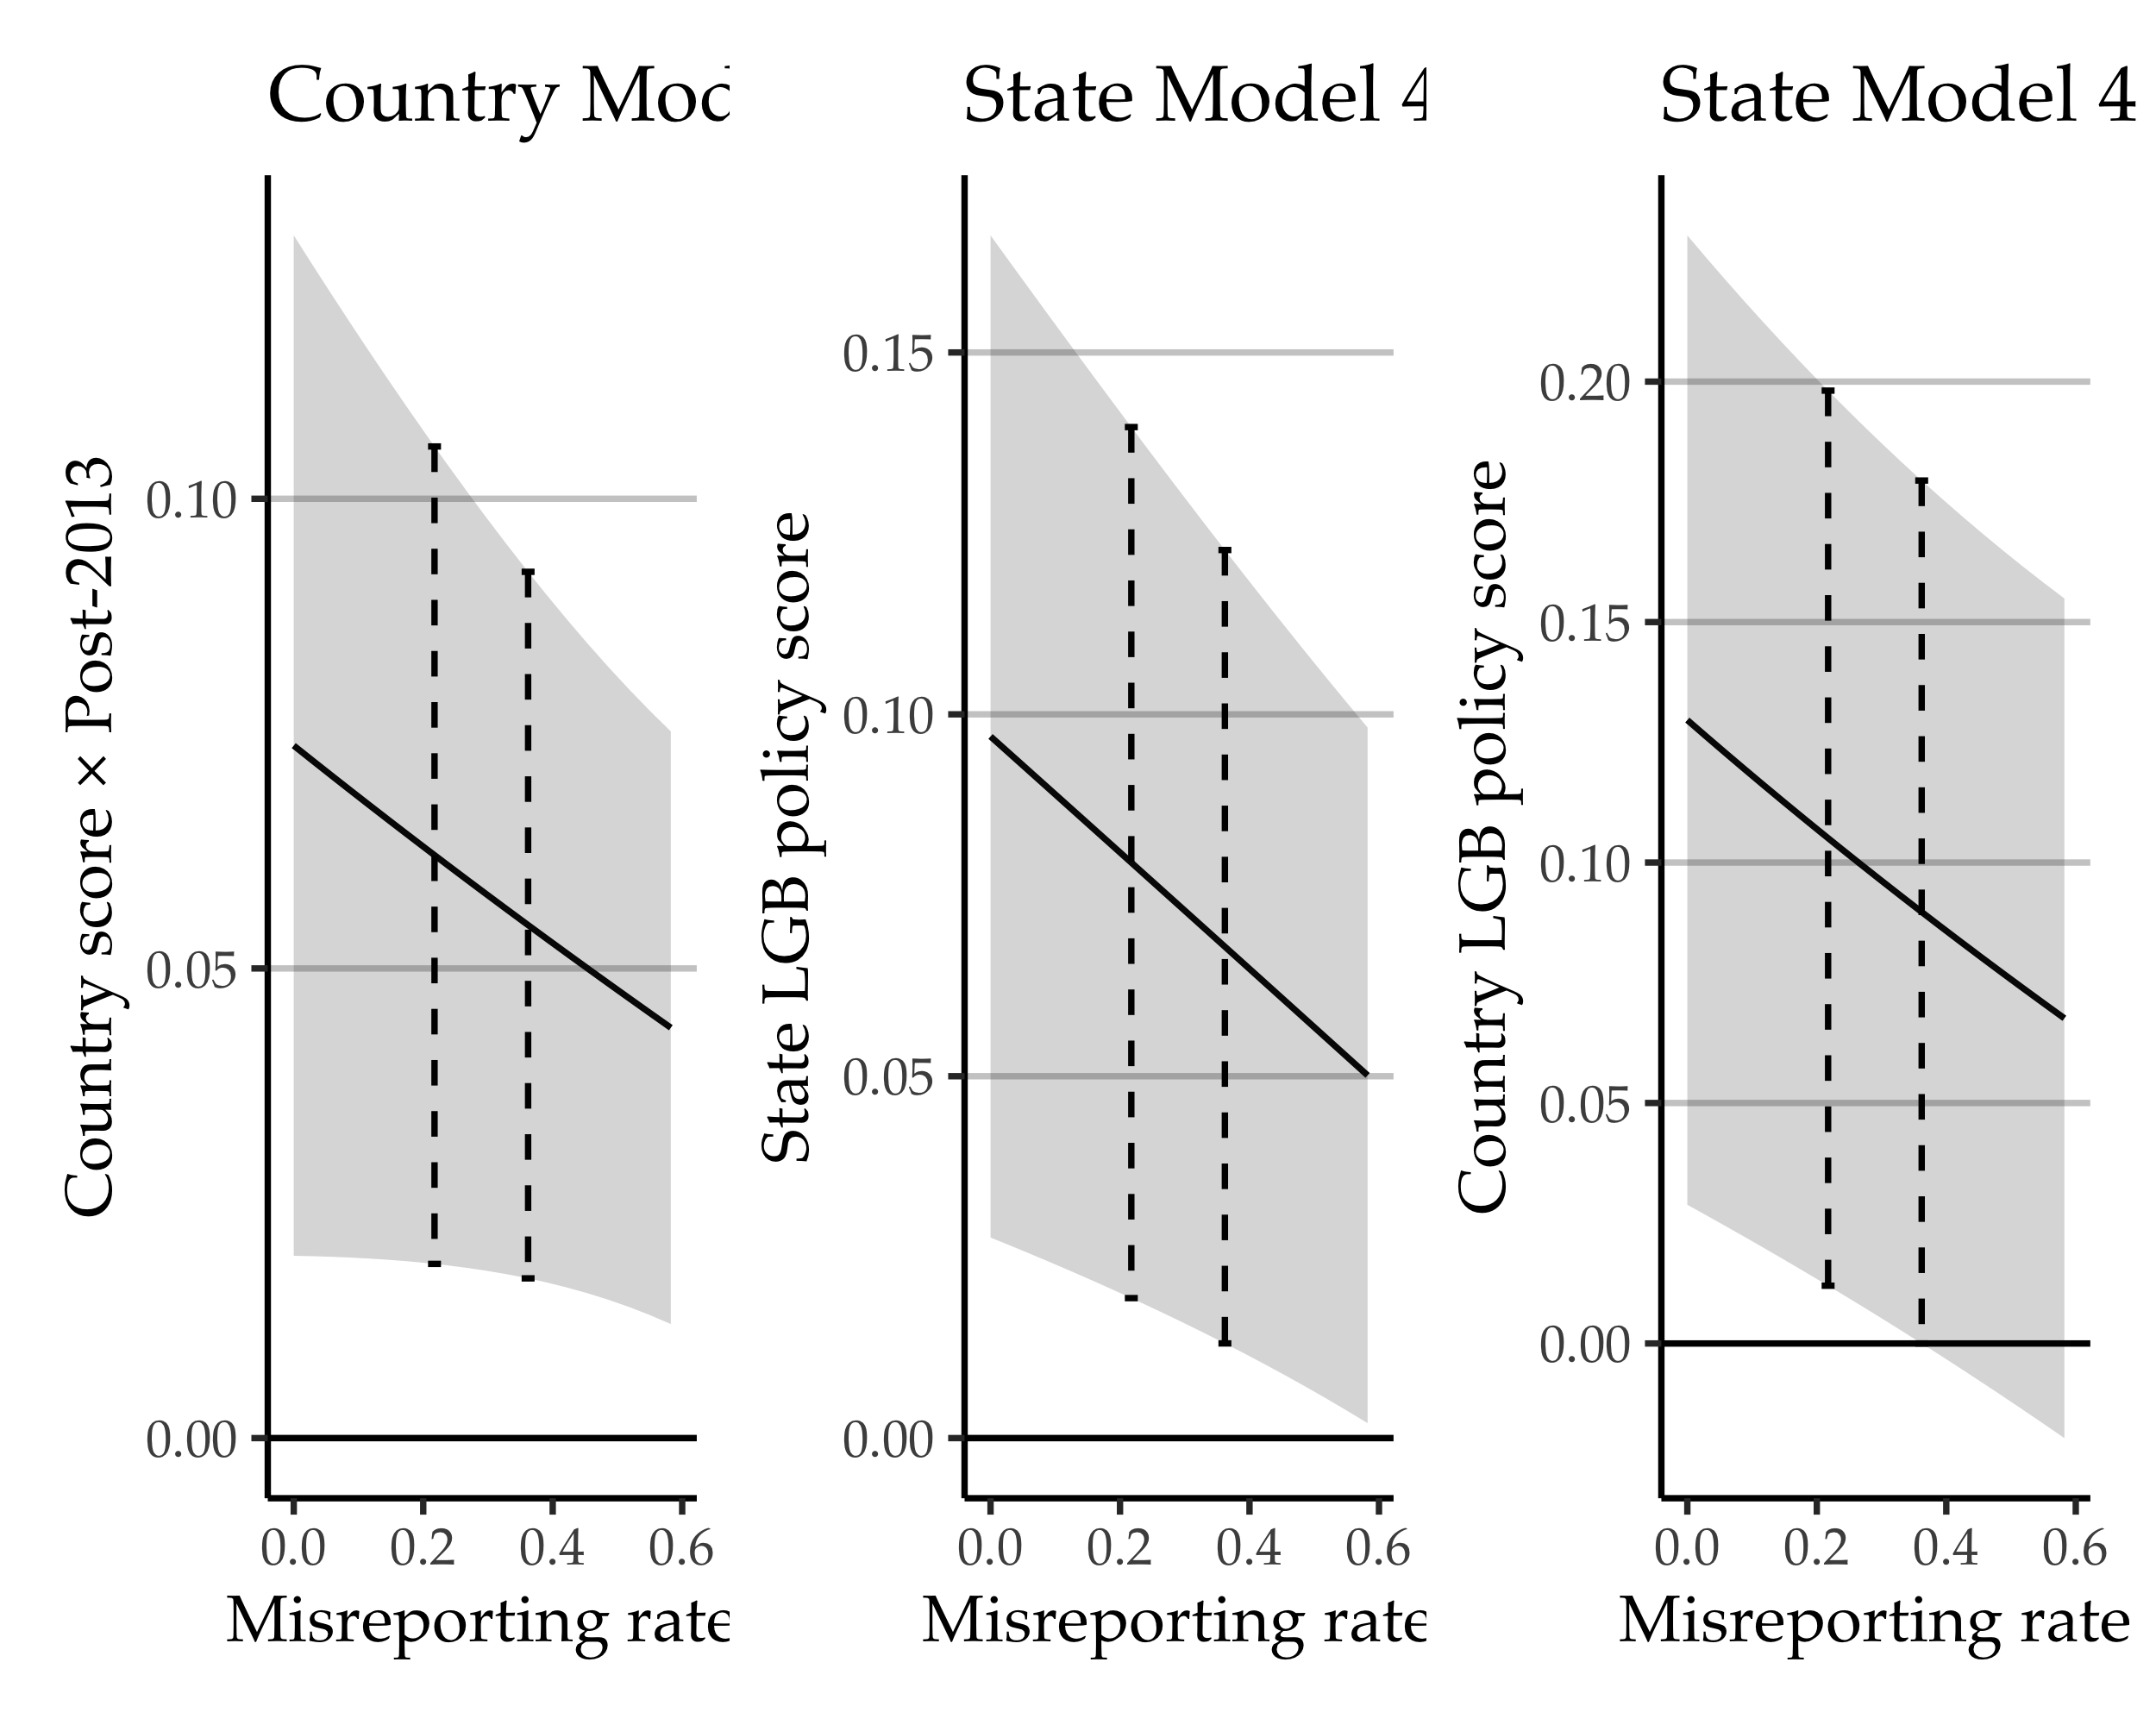
\includegraphics{ssimm_supp_small_files/figure-latex/sens-1.pdf}
\caption{\label{fig:sens}Coefficient for sending-country LGBT policy context for fixed effects models, adjusted for possible misreporting of same-sex couples in pre-2019 data. Ribbon shows 95 percent confidence intervals and blue bars show estimated misreporting from the 2010 and 2016 U.S. Census Bureau tests on the ACS.}
\end{figure}

\newpage

\hypertarget{references}{%
\section{References}\label{references}}

\setlength{\parindent}{-0.2in}
\setlength{\leftskip}{0.2in}
\setlength{\parskip}{8pt}

\noindent

\hypertarget{refs}{}
\begin{CSLReferences}{1}{0}
\leavevmode\hypertarget{ref-gates_2009}{}%
Gates, G. J., \& Steinberger, M. D. (2009). Same-sex unmarried partner couples in the {American Community Survey}: {The} role of misreporting, miscoding and misallocation. \emph{Annual Meetings of the Population Association of America, Detroit, {MI}}.

\leavevmode\hypertarget{ref-kreider_2017}{}%
Kreider, R. M., Bates, N., \& Mayol-García, Y. (2017). Improving measurement of same-sex couple households in {Census Bureau} surveys: {Results} from recent tests. \emph{{PAA} 2017 Annual Meeting}.

\leavevmode\hypertarget{ref-kreider_2015}{}%
Kreider, R. M., \& Lofquist, D. A. (2015). \emph{Matching survey data with administrative records to evaluate reports of same-sex married couple households} (SEHSD Working Paper No. 2019-30).

\leavevmode\hypertarget{ref-u.s.censusbureau_2017}{}%
U.S. Census Bureau. (2017). \emph{American {Community Survey Information Guide}}. {U.S. Census Bureau}.

\leavevmode\hypertarget{ref-walker_2021}{}%
Walker, L., \& Taylor, D. (2021). \emph{Same-{Sex Couple Households}: 2019} (American Community Survey Briefs ACSBR-005). {U.S. Census Bureau}.

\end{CSLReferences}

\end{document}
